% =====================================================================
%  Campus Event Management Platform: project report (CS 202C)
%  Build:  ./scripts/build_docs.sh      (or upload report/ to Overleaf)
% =====================================================================
\documentclass[11pt,a4paper]{article}

% ---------- Packages ----------
\usepackage[T1]{fontenc}
\usepackage[utf8]{inputenc}
\usepackage{lmodern}
\usepackage{microtype}
\usepackage[margin=2.4cm]{geometry}
\usepackage{graphicx}
\usepackage{booktabs}
\usepackage{array}
\usepackage{tabularx}
\usepackage{float}
\usepackage{caption}
\usepackage{enumitem}
\usepackage{xcolor}
\usepackage{listings}
\usepackage{tikz}
\usetikzlibrary{positioning,arrows.meta,fit,shapes.geometric}
\usepackage{pgfplots}
\pgfplotsset{compat=1.17}
\usepackage{hyperref}   % load last
\hypersetup{colorlinks=true, linkcolor=blue!50!black, urlcolor=blue!50!black, citecolor=blue!50!black}

% ---------- Helper commands ----------
% \code{...}: inline code; \detokenize lets us write underscores directly.
\newcommand{\code}[1]{\texttt{\detokenize{#1}}}
% Red reminder for things only the author can fill in. Remove before submitting.
\newcommand{\todo}[1]{\textcolor{red}{\textbf{[TODO: #1]}}}
% \screenshot{file}{width}{what to capture}: shows the image if the file exists,
% otherwise a box telling you which screenshot to take.
\newcommand{\screenshot}[3]{%
  \IfFileExists{#1}{\includegraphics[width=#2]{#1}}{%
    \fbox{\parbox[c][3.5cm][c]{0.8\linewidth}{\centering\small
      Screenshot missing: save it as \texttt{report/\detokenize{#1}}\\[4pt]
      (#3)}}}}

% ---------- Code listing style ----------
\definecolor{codebg}{RGB}{246,248,250}
\lstset{
  basicstyle=\ttfamily\footnotesize,
  backgroundcolor=\color{codebg},
  frame=single, rulecolor=\color{black!20},
  breaklines=true, columns=fullflexible, keepspaces=true,
  showstringspaces=false, tabsize=4, captionpos=b,
  keywordstyle=\color{blue!70!black}\bfseries,
  commentstyle=\color{green!40!black}\itshape,
  stringstyle=\color{red!60!black},
}

\begin{document}

% =====================================================================
\begin{titlepage}
  \centering
  \vspace*{2.5cm}
  {\Huge\bfseries Campus Event Management Platform\par}
  \vspace{0.6cm}
  {\Large A Flask and SQLite web application\\ with profiling-driven optimisation\par}
  \vspace{2.5cm}
  {\Large Prajyot\par}
  \vspace{0.3cm}
  {\large \todo{roll number}\par}
  \vspace{1.5cm}
  {\large Course: CS 202C\par}
  \vspace{0.2cm}
  {\large Indian Institute of Technology Dharwad\par}
  \vfill
  {\large November 2026\par}
\end{titlepage}

% =====================================================================
\begin{abstract}
This report describes the Campus Event Management Platform, a web application in
which students browse, search and register for campus events and administrators manage
events, venues, participant lists and reports. It is built with Python and Flask, uses
SQLite through raw SQL, is styled with hand-written HTML and CSS, is automated with Bash
scripts and versioned with Git. The application is covered by 45 automated pytest tests.
A deliberately naive first version of the reports page was profiled with \code{cProfile} on
2000 events and 67{,}423 registrations: 99\% of the time was spent in 6000 small SQL
queries (the \emph{N+1 query problem}). Rewriting each report as one \code{JOIN}~+~\code{GROUP BY}
query and adding three indexes reduced the total time from 10.9\,s to 32.6\,ms (about
335$\times$ faster) and the number of SQL statements from 6016 to 6, while the tests
confirmed that every report number stayed the same.
\end{abstract}

\tableofcontents
\newpage

% =====================================================================
\section{Introduction and objectives}

Colleges run many events: technical talks, cultural nights, sports matches, workshops and
seminars. Information about them is often scattered across posters and chat groups, sign-ups
are collected in spreadsheets, and nobody knows how full an event is or whether two events
have been booked into the same hall at the same time.

The goal of this project is a small but complete web application that solves these problems,
built so that every line can be explained. The objectives were:

\begin{enumerate}[itemsep=2pt]
  \item Let \textbf{students} create an account, browse upcoming events, search and filter
        them, and register or cancel, with the app enforcing capacity limits.
  \item Let \textbf{admins} create, edit and delete events and venues, with the app
        rejecting \textbf{venue time clashes}, and view and export participant lists.
  \item Give admins a \textbf{reports} page: registrations and fill rate per event, popular
        categories and venue utilisation.
  \item Use at least five course modules (HTML/CSS, Python, SQL, Git, Bash), plus LaTeX for
        this report and the slides.
  \item Back the code with \textbf{automated tests} and use a \textbf{profiler} to find and fix
        a real performance bottleneck, with measured before/after results.
  \item Keep the code simple and well commented, with no ORM and no CSS framework, so that the
        SQL and CSS are written and understood by hand.
\end{enumerate}

% =====================================================================
\section{Course modules used}

\begin{table}[H]
\centering
\small
\begin{tabularx}{\linewidth}{@{}l X@{}}
\toprule
\textbf{Module} & \textbf{Where and how it is used} \\
\midrule
HTML/CSS & 16 Jinja2 templates in \code{app/templates/} that extend one \code{base.html}
           layout; one hand-written stylesheet \code{app/static/style.css} using CSS custom
           properties (variables), flexbox, CSS grid and horizontally scrolling tables for phones.
           The fill-rate bars on the reports page are pure CSS. \\
Python   & Flask application factory, three Blueprints (\code{auth}, \code{events},
           \code{admin}), Flask-Login sessions, Werkzeug password hashing, the \code{csv}
           module for export, a Faker-based seed command, pytest tests, and the
           \code{cProfile}/\code{pstats} profiling scripts. \\
SQL      & Raw SQL through Python's built-in \code{sqlite3} module: table definitions with
           \code{PRIMARY KEY}, \code{UNIQUE}, \code{CHECK}, \code{FOREIGN KEY} and
           \code{ON DELETE CASCADE}; parameterised queries with \code{?}; \code{LEFT JOIN},
           \code{GROUP BY}, \code{COUNT(DISTINCT)}, sub-queries and derived tables;
           indexes; \code{EXPLAIN QUERY PLAN}. \\
Git      & 23 small commits (before this documentation phase) following a
           \code{type: message} convention; \code{.gitignore} and \code{.gitattributes}. \\
Bash     & Seven scripts in \code{scripts/} for setup, running, seeding, testing, profiling
           and building the documents, all with \code{set -euo pipefail} and working in Git
           Bash on Windows as well as on Linux/macOS. \\
LaTeX    & This report (TikZ diagrams, \code{listings} code, a \code{pgfplots} chart) and the
           Beamer slides. \\
\bottomrule
\end{tabularx}
\caption{Course modules and where they appear in the project.}
\end{table}

% =====================================================================
\section{System architecture}

The application follows the classic three-tier pattern: the browser sends HTTP requests,
Flask decides which Python function handles each URL, the function reads or writes the
SQLite database with SQL, and the result is rendered into HTML by a Jinja2 template.
Figure~\ref{fig:arch} shows the parts.

\begin{figure}[H]
\centering
\resizebox{\linewidth}{!}{%
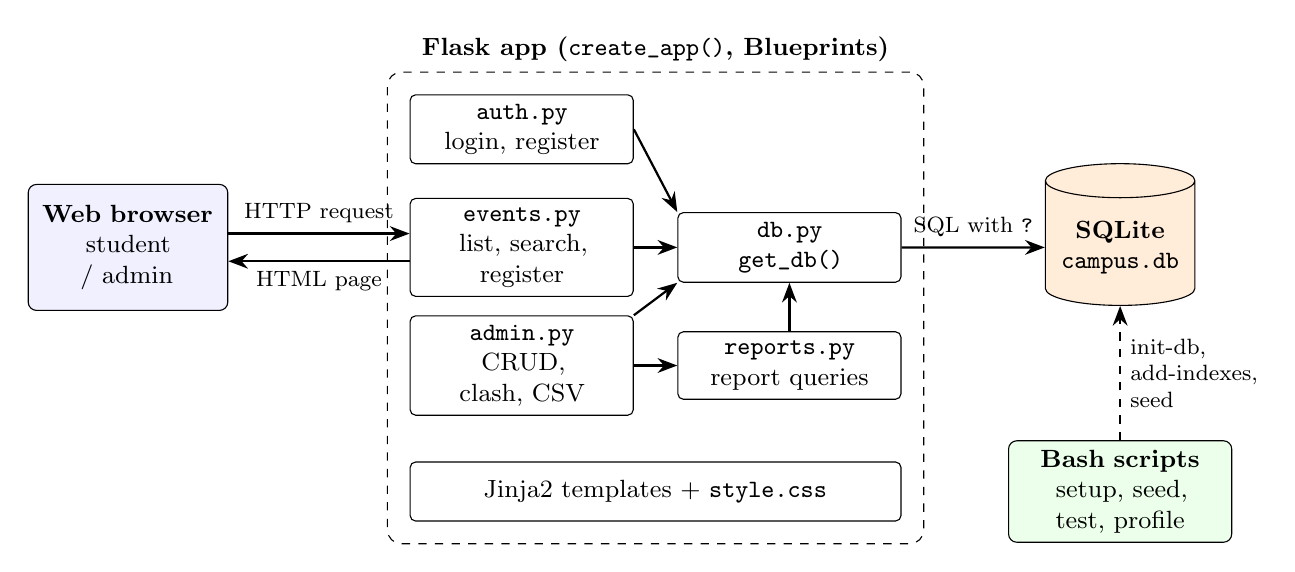
\begin{tikzpicture}[
    font=\small,
    box/.style={draw, rounded corners=3pt, fill=blue!6, align=center, minimum height=0.9cm, text width=2.5cm},
    mod/.style={draw, rounded corners=2pt, fill=white, align=center, minimum height=0.75cm, text width=2.6cm},
    arr/.style={-{Stealth[length=2.5mm]}, thick},
  ]
  \node[box, text width=2.3cm, minimum height=1.6cm] (browser) at (0,0) {\textbf{Web browser}\\ student / admin};

  \node[mod] (auth)   at (5,1.5)  {\code{auth.py}\\ login, register};
  \node[mod] (events) at (5,0)    {\code{events.py}\\ list, search, register};
  \node[mod] (admin)  at (5,-1.5) {\code{admin.py}\\ CRUD, clash, CSV};
  \node[mod] (reports) at (8.4,-1.5) {\code{reports.py}\\ report queries};
  \node[mod] (db)     at (8.4,0)  {\code{db.py}\\ \code{get_db()}};
  \node[mod, text width=6cm] (tpl) at (6.7,-3.1) {Jinja2 templates + \code{style.css}};

  \node[draw, dashed, rounded corners=5pt, inner sep=8pt, fit=(auth)(admin)(reports)(db)(tpl),
        label={[font=\small\bfseries]above:Flask app (\code{create_app()}, Blueprints)}] (flask) {};

  \node[draw, shape=cylinder, shape border rotate=90, aspect=0.25, fill=orange!15,
        minimum height=1.8cm, minimum width=1.9cm, align=center] (sqlite) at (12.6,0)
        {\textbf{SQLite}\\ \code{campus.db}};

  \node[box, fill=green!8, text width=2.6cm] (bash) at (12.6,-3.1)
        {\textbf{Bash scripts}\\ setup, seed, test, profile};

  % browser and events.py are both at y = 0, so these arrows are horizontal
  \draw[arr] ([yshift=5pt]browser.east) -- node[above, font=\footnotesize]{HTTP request} ([yshift=5pt]events.west);
  \draw[arr] ([yshift=-5pt]events.west) -- node[below, font=\footnotesize]{HTML page} ([yshift=-5pt]browser.east);
  \draw[arr] (auth.east)   -- (db.north west);
  \draw[arr] (events.east) -- (db.west);
  \draw[arr] (admin.east)  -- (reports.west);
  \draw[arr] (admin.north east) -- (db.south west);
  \draw[arr] (reports.north) -- (db.south);
  \draw[arr] (db.east) -- node[above, font=\footnotesize]{SQL with \code{?}} (sqlite.west);
  \draw[arr, dashed] (bash.north) -- node[right, font=\footnotesize, align=left]{init-db,\\ add-indexes,\\ seed} (sqlite.south);
\end{tikzpicture}}
\caption{Architecture: browser $\rightarrow$ Flask Blueprints $\rightarrow$ SQLite.}
\label{fig:arch}
\end{figure}

\paragraph{Application factory.} \code{create_app()} in \code{app/__init__.py} builds the Flask
app, sets the secret key and database path, registers the Blueprints, sets up Flask-Login
and adds friendly 403/404 error pages. Building the app inside a function lets the tests
create a fresh app that points at a temporary database.

\paragraph{Blueprints.} Each Blueprint groups related routes in its own file:
\code{auth} (\code{/auth/...}), \code{events} (\code{/events/...} and \code{/my-registrations})
and \code{admin} (\code{/admin/...}). Calculations that need to be tested or profiled on their
own, such as \code{search_events()}, \code{find_clash()} and the report functions, are plain
Python functions rather than routes.

\paragraph{Database access.} \code{get_db()} opens one SQLite connection per request and stores
it in Flask's \code{g} object; \code{close_db()} closes it when the request ends. Each connection
runs \code{PRAGMA foreign_keys = ON}, because SQLite does not enforce foreign keys unless asked.

\paragraph{Security basics.} Passwords are stored only as salted hashes
(\code{generate_password_hash}). Every SQL value is passed through a \code{?} placeholder, which
prevents SQL injection. Jinja2 escapes all output, which prevents HTML injection. Every action that
changes data is a \code{POST} form, and the session cookie uses \code{SameSite=Lax} so other websites
cannot submit those forms on a logged-in user's behalf.

% =====================================================================
\section{Database design}

\begin{figure}[H]
\centering
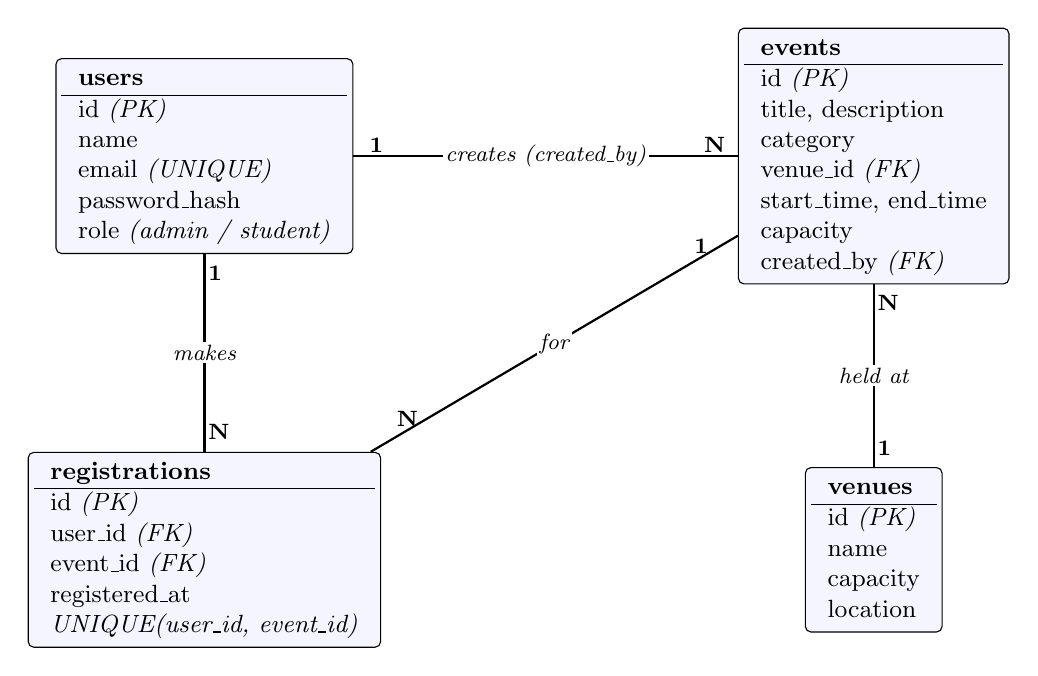
\begin{tikzpicture}[
    entity/.style={draw, rounded corners=2pt, fill=blue!4, font=\small, inner sep=2pt},
    rel/.style={draw, thick},
    card/.style={font=\footnotesize\bfseries, inner sep=1pt},
    lbl/.style={font=\footnotesize\itshape, fill=white, inner sep=1pt},
  ]
  \node[entity] (users) at (0,0) {\begin{tabular}{l}
    \textbf{users}\\ \hline
    id \textit{(PK)}\\
    name\\
    email \textit{(UNIQUE)}\\
    password\_hash\\
    role \textit{(admin / student)}
  \end{tabular}};

  \node[entity] (events) at (8.5,0) {\begin{tabular}{l}
    \textbf{events}\\ \hline
    id \textit{(PK)}\\
    title, description\\
    category\\
    venue\_id \textit{(FK)}\\
    start\_time, end\_time\\
    capacity\\
    created\_by \textit{(FK)}
  \end{tabular}};

  \node[entity] (regs) at (0,-5) {\begin{tabular}{l}
    \textbf{registrations}\\ \hline
    id \textit{(PK)}\\
    user\_id \textit{(FK)}\\
    event\_id \textit{(FK)}\\
    registered\_at\\
    \textit{UNIQUE(user\_id, event\_id)}
  \end{tabular}};

  \node[entity] (venues) at (8.5,-5) {\begin{tabular}{l}
    \textbf{venues}\\ \hline
    id \textit{(PK)}\\
    name\\
    capacity\\
    location
  \end{tabular}};

  \draw[rel] (users) -- node[lbl]{creates (created\_by)}
      node[card, pos=0.06, above]{1} node[card, pos=0.94, above]{N} (events);
  \draw[rel] (users) -- node[lbl]{makes}
      node[card, pos=0.1, right]{1} node[card, pos=0.9, right]{N} (regs);
  \draw[rel] (regs) -- node[lbl]{for}
      node[card, pos=0.1, above]{N} node[card, pos=0.9, above]{1} (events);
  \draw[rel] (events) -- node[lbl]{held at}
      node[card, pos=0.1, right]{N} node[card, pos=0.9, right]{1} (venues);
\end{tikzpicture}
\caption{Entity--relationship diagram. \texttt{registrations} is the link table for the
many-to-many relationship between students and events.}
\label{fig:er}
\end{figure}

The schema (\code{sql/schema.sql}) has four tables:

\begin{itemize}[itemsep=2pt]
  \item \textbf{users}: everyone who can log in. \code{email} is \code{UNIQUE}, and \code{role} has a
        \code{CHECK (role IN ('admin','student'))} constraint, so the database itself rejects any
        other value.
  \item \textbf{venues}: physical rooms, with \code{CHECK (capacity > 0)}.
  \item \textbf{events}: each event belongs to one venue (\code{venue_id}) and one creator
        (\code{created_by}). A table-level \code{CHECK (end_time > start_time)} makes events that
        end before they start impossible.
  \item \textbf{registrations}: the link table between students and events.
        \code{UNIQUE (user_id, event_id)} means a student can register for an event only once,
        even if the application code had a bug. \code{ON DELETE CASCADE} removes an event's
        registrations automatically when the event is deleted.
\end{itemize}

\begin{lstlisting}[language=SQL, caption={The registrations table in sql/schema.sql.}]
CREATE TABLE registrations (
    id            INTEGER PRIMARY KEY AUTOINCREMENT,
    user_id       INTEGER NOT NULL REFERENCES users(id)  ON DELETE CASCADE,
    event_id      INTEGER NOT NULL REFERENCES events(id) ON DELETE CASCADE,
    registered_at TEXT    NOT NULL DEFAULT (datetime('now', 'localtime')),
    UNIQUE (user_id, event_id)   -- a student can register only once per event
);
\end{lstlisting}

\paragraph{Dates as text.} Times are stored as \code{TEXT} in ISO format
\code{'YYYY-MM-DD HH:MM'}. Because the most significant part comes first, comparing two such
strings alphabetically gives the same answer as comparing the times. So \code{<}, \code{>} and
\code{ORDER BY} work directly, which the clash check relies on.

\paragraph{Indexes.} The schema deliberately started without extra indexes. They were added
later in a separate file, \code{sql/indexes.sql}, as the result of profiling
(Section~\ref{sec:profiling}).

% =====================================================================
\section{Features and implementation}

\subsection{Authentication and roles}

Students register through a form; the role is always fixed to \code{'student'} in the
\code{INSERT}, so nobody can sign up as an admin (the admin account is created by
\code{setup.sh}). A duplicate email raises \code{sqlite3.IntegrityError} from the
\code{UNIQUE} constraint, which is caught and shown as a friendly message. Login uses
\code{check_password_hash}, and the same message is shown for an unknown email and a wrong
password so that attackers cannot find out which emails exist. Flask-Login keeps the user's id in a
signed session cookie and turns it back into a \code{User} object on each request.

Admin-only pages are protected by a small decorator:

\begin{lstlisting}[language=Python, caption={The admin\_required decorator in app/auth.py.}]
def admin_required(view):
    @functools.wraps(view)  # keep the original function's name for Flask's routing
    def wrapped_view(*args, **kwargs):
        if not current_user.is_authenticated:
            return login_manager.unauthorized()   # -> redirect to login page
        if not current_user.is_admin:
            abort(403)                            # logged in, but not an admin
        return view(*args, **kwargs)
    return wrapped_view
\end{lstlisting}

\subsection{Browsing and searching events}

The events page lists upcoming events with the venue name and the number of seats left
(\code{capacity - COUNT(r.id)}). The search form has a keyword, a category dropdown, a venue
dropdown and a date range. It uses \code{GET}, so filters appear in the URL and a search can be
bookmarked. The \code{WHERE} clause is built from two lists: \code{conditions} only ever holds
fixed SQL text written by the programmer, and \code{params} holds the user's input, which reaches
SQLite only through \code{?} placeholders.

\begin{lstlisting}[language=Python, caption={Building the search query safely (app/events.py, shortened).}]
conditions = ["e.start_time >= ?"]   # only upcoming events
params = [now_string()]
if keyword:
    conditions.append("(e.title LIKE ? OR e.description LIKE ?)")
    pattern = f"%{keyword}%"         # % means "any text" in LIKE
    params.extend([pattern, pattern])
if category:
    conditions.append("e.category = ?")
    params.append(category)
# ... venue_id, date_from and date_to are added the same way ...
sql = ("SELECT e.id, e.title, ..., e.capacity - COUNT(r.id) AS seats_left "
       "FROM events e JOIN venues v ON v.id = e.venue_id "
       "LEFT JOIN registrations r ON r.event_id = e.id "
       "WHERE " + " AND ".join(conditions) + " "
       "GROUP BY e.id ORDER BY e.start_time")
\end{lstlisting}

Typing \code{' OR 1=1 --} into the search box therefore finds nothing: it is treated as
ordinary text to search for, not as SQL.

\begin{figure}[H]
\centering
\screenshot{figures/search_page.png}{0.85\linewidth}{Events page with a keyword and category filter applied}
\caption{Searching and filtering upcoming events.}
\end{figure}

\subsection{Registering and cancelling}

Registration is a \code{POST} request from the button on the event detail page. The route checks
every reason to refuse, in order, and explains which one applied:

\begin{lstlisting}[language=Python, caption={Registration rules in register\_for\_event() (app/events.py).}]
if current_user.is_admin:
    flash("Admins cannot register for events.", "error")
elif event["start_time"] <= now_string():
    flash("This event has already started.", "error")
elif is_registered(current_user.id, event_id):
    flash("You are already registered for this event.", "error")
elif event["seats_left"] <= 0:
    flash("Sorry, this event is full.", "error")
else:
    conn.execute("INSERT INTO registrations (user_id, event_id) VALUES (?, ?)",
                 (current_user.id, event_id))
    conn.commit()
    flash(f"You are registered for {event['title']}.", "success")
\end{lstlisting}

Cancelling runs \code{DELETE FROM registrations WHERE user_id = ? AND event_id = ?} and uses
\code{cursor.rowcount} to tell whether anything was actually deleted. The \textbf{My registrations}
page joins \code{registrations}, \code{events} and \code{venues} for the logged-in student's
upcoming events.

\begin{figure}[H]
\centering
\begin{minipage}{0.48\linewidth}\centering
\screenshot{figures/detail_page.png}{\linewidth}{Event detail page with the Register button}
\end{minipage}\hfill
\begin{minipage}{0.48\linewidth}\centering
\screenshot{figures/my_registrations_page.png}{\linewidth}{My registrations page}
\end{minipage}
\caption{Event detail page (left) and a student's registrations (right).}
\end{figure}

\subsection{Admin: venues, events and the clash check}

Admins can create, edit and delete venues and events. New and edit share one form and one
validation function, \code{read_event_form()}, which checks that the title and category are
present, the times are valid, the event ends after it starts, the capacity is positive and not
larger than the venue's capacity, and (when editing) not smaller than the number of students
already registered. Finally it calls the clash check:

\begin{lstlisting}[language=Python, caption={Venue clash check in app/admin.py.}]
def find_clash(venue_id, start_time, end_time, ignore_event_id=None):
    """Return the first event at this venue whose time overlaps, or None.
    Two ranges overlap when each one starts before the other one ends."""
    sql = ("SELECT id, title, start_time, end_time FROM events "
           "WHERE venue_id = ? AND start_time < ? AND end_time > ?")
    params = [venue_id, end_time, start_time]
    if ignore_event_id is not None:      # when editing, skip the event itself
        sql += " AND id != ?"
        params.append(ignore_event_id)
    return get_db().execute(sql + " LIMIT 1", params).fetchone()
\end{lstlisting}

Two events that only touch (one ends at 11:00, the next starts at 11:00) do not clash, because
the comparisons are strict. When an event is edited, its own id is excluded; otherwise every edit
would clash with itself. The form uses HTML \code{datetime-local} inputs, whose
\code{2026-11-20T14:30} value is converted to the database format by \code{to_db_time()}.

\begin{figure}[H]
\centering
\screenshot{figures/clash_error_page.png}{0.85\linewidth}{New event form showing the "already booked" clash error}
\caption{Creating an event that overlaps another event at the same venue is rejected.}
\end{figure}

\subsection{Participants and CSV export}

\code{/admin/events/<id>/participants} lists each participant's name, email and registration
time. The \textbf{Export CSV} button returns the same rows written with Python's \code{csv.writer}
into an in-memory \code{io.StringIO} buffer. A \code{Content-Disposition: attachment} header
makes the browser download the file instead of displaying it. \code{csv.writer} takes care of
commas and quotes inside names.

\subsection{Reports}

The reports page (Figures~\ref{fig:reports1} and~\ref{fig:reports2}) shows popular categories,
venue utilisation (registrations as a percentage of the seats offered by the venue's events) and
registrations with fill rate for every event. The calculations live in \code{app/reports.py} so
that tests and the profiler can call them directly. How they were made fast is the subject of
Section~\ref{sec:profiling}.

\begin{figure}[H]
\centering
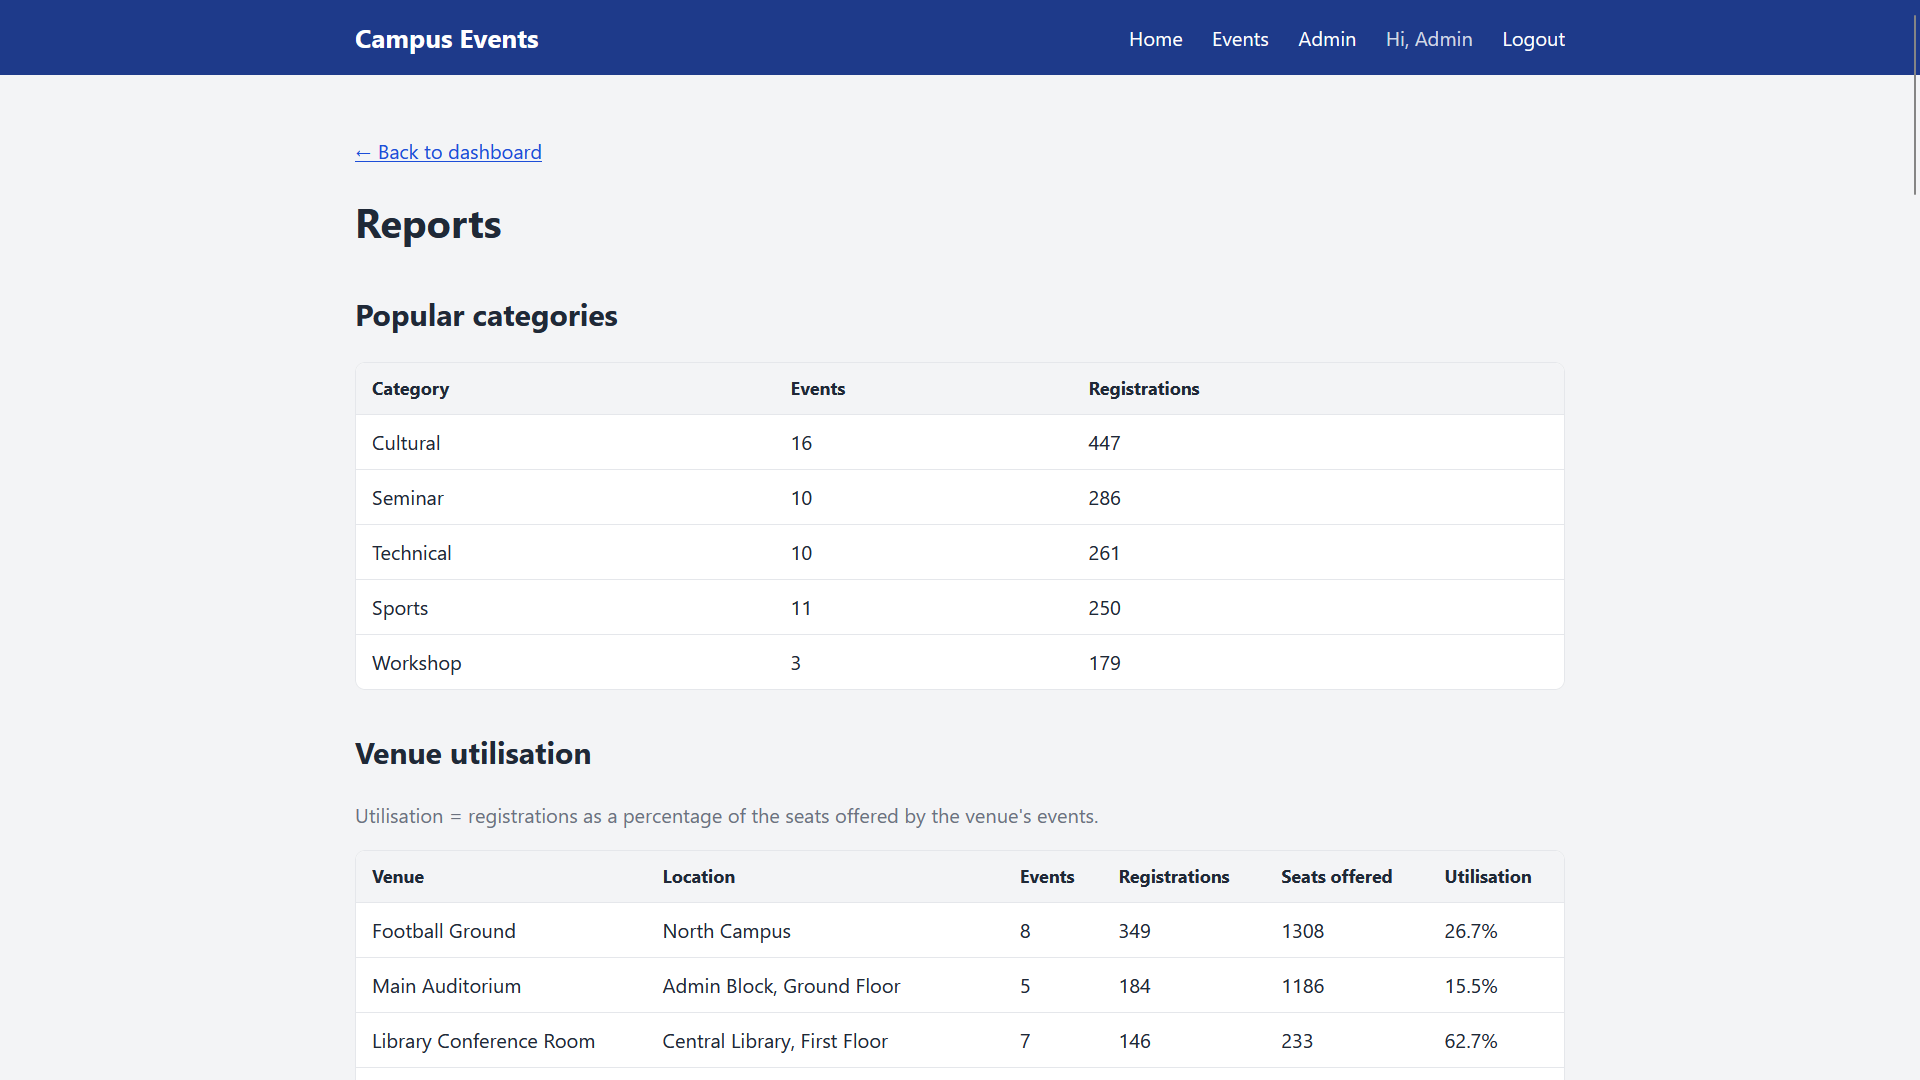
\includegraphics[width=0.85\linewidth]{figures/events_search.png}
\caption{Reports page: popular categories and venue utilisation (demo data, 50 events).}
\label{fig:reports1}
\end{figure}

\begin{figure}[H]
\centering
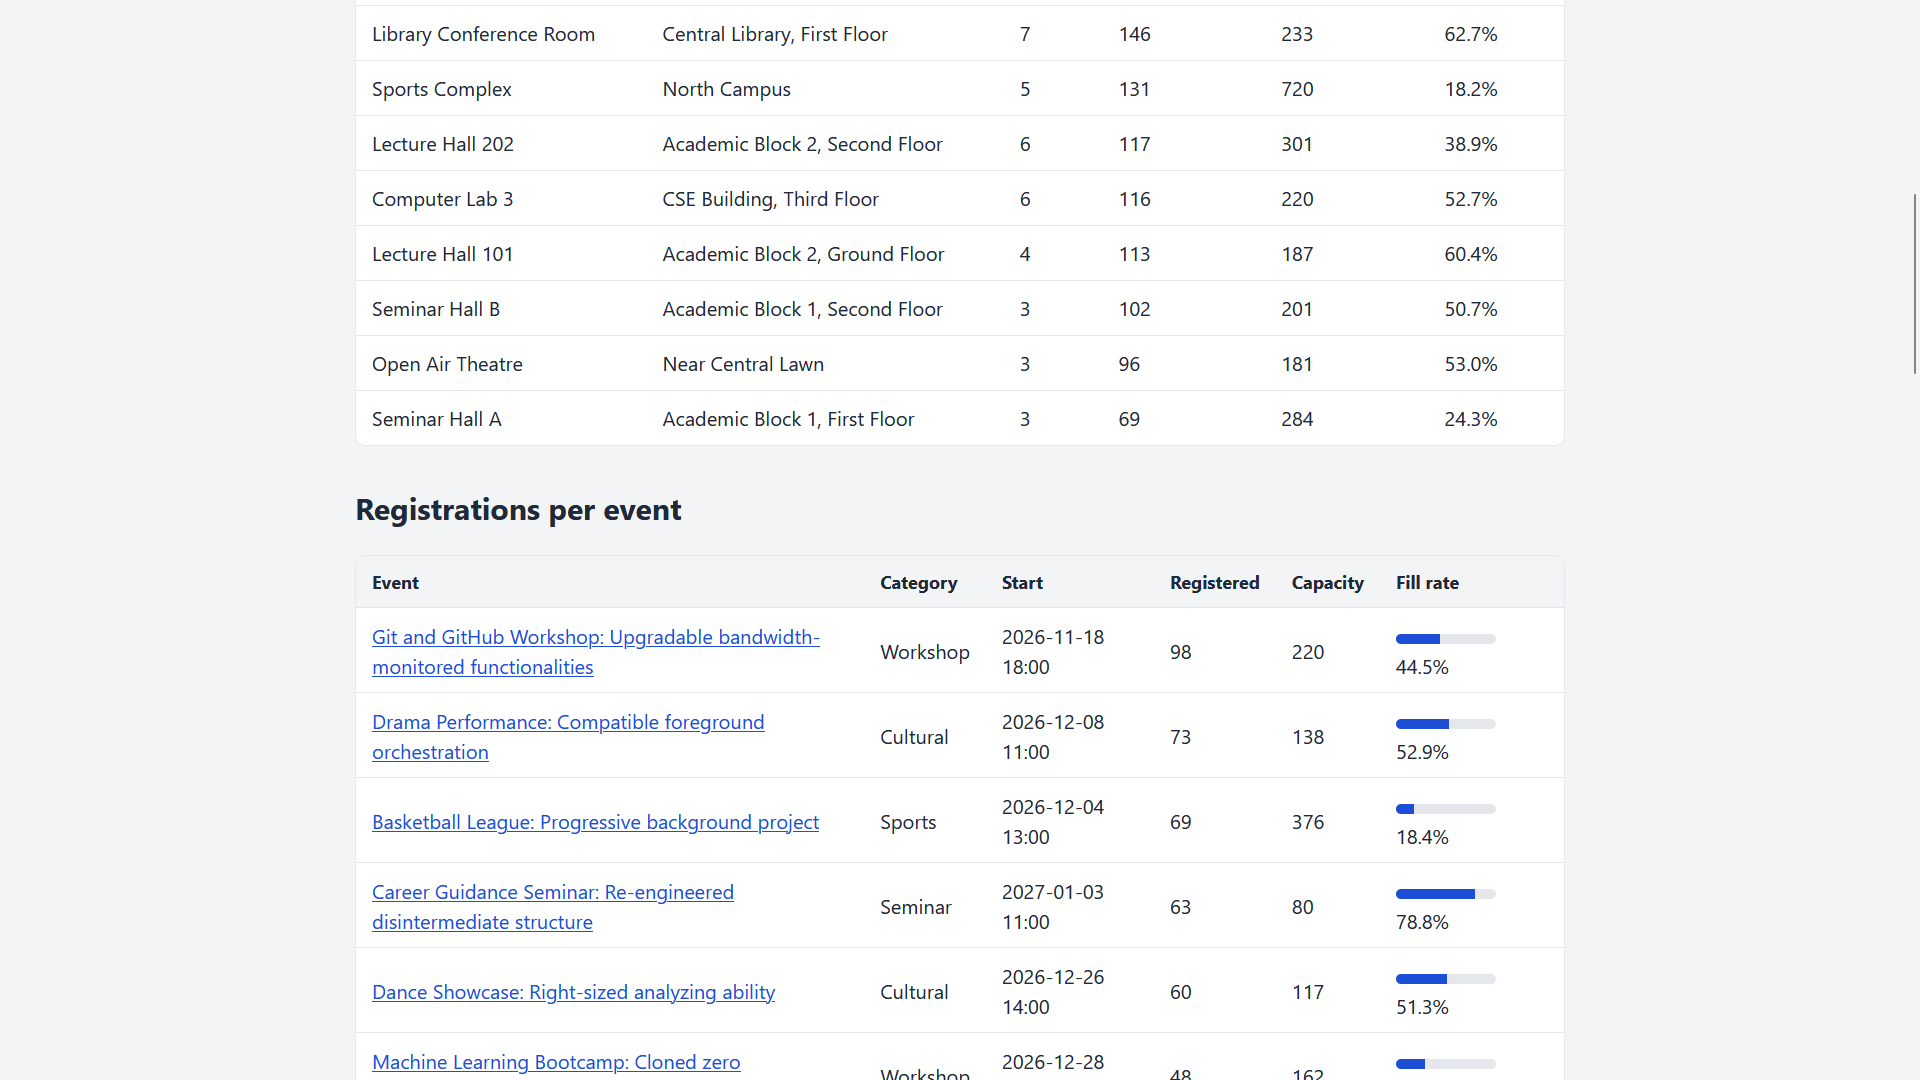
\includegraphics[width=0.85\linewidth]{figures/admin_events.png}
\caption{Reports page: rest of venue utilisation and registrations per event with CSS fill-rate bars.}
\label{fig:reports2}
\end{figure}

% =====================================================================
\section{Bash automation}

Every routine task has a script. All of them start with \code{set -euo pipefail}: \code{-e}
stops on the first failing command, \code{-u} treats unset variables as errors, and
\code{pipefail} makes a pipeline fail if any part fails. They share helper functions from
\code{scripts/common.sh}.

\begin{table}[H]
\centering
\small
\begin{tabularx}{\linewidth}{@{}l X@{}}
\toprule
\textbf{Script} & \textbf{What it does} \\
\midrule
\code{setup.sh}      & Finds a working Python, creates \code{venv/}, installs requirements, creates the database, adds indexes, creates the admin (login can be changed with \code{ADMIN_EMAIL} / \code{ADMIN_PASSWORD}). \\
\code{run.sh}        & Activates the venv, checks the database exists, starts Flask in debug mode (\code{PORT} can be changed). \\
\code{seed.sh [N]}   & Validates N with a regular expression (\code{^[0-9]+$}) and fills the database with Faker data. \\
\code{test.sh}       & Runs \code{pytest -v}; extra arguments are passed on with \code{"$@"}. \\
\code{profile.sh}    & Builds a separate profiling database (\code{CAMPUS_DB}), seeds it, optionally adds indexes (\code{APPLY_INDEXES}), runs the profiler and saves the query plans. \\
\code{build_docs.sh} & Compiles this report and the slides if LaTeX is installed. \\
\code{common.sh}     & Shared functions \code{find_python} and \code{activate_venv}. \\
\bottomrule
\end{tabularx}
\caption{Automation scripts in \texttt{scripts/}.}
\end{table}

The scripts had to work in Git Bash on Windows as well as on Linux/macOS. Two details matter:
a Windows virtual environment keeps its activate script in \code{venv/Scripts/} instead of
\code{venv/bin/}, and on Windows \code{python3} can be a Microsoft Store shortcut that exists but
only prints an error. So the helper actually \emph{runs} each candidate:

\begin{lstlisting}[language=bash, caption={Finding a working Python and activating the venv (scripts/common.sh).}]
find_python() {
    if python3 --version >/dev/null 2>&1; then
        PYTHON="python3"
    elif python --version >/dev/null 2>&1; then
        PYTHON="python"
    else
        echo "ERROR: Python 3 was not found."; exit 1
    fi
}

activate_venv() {
    if [ -f "$VENV_DIR/Scripts/activate" ]; then      # Windows
        ACTIVATE="$VENV_DIR/Scripts/activate"
    elif [ -f "$VENV_DIR/bin/activate" ]; then        # Linux / macOS
        ACTIVATE="$VENV_DIR/bin/activate"
    else
        echo "ERROR: run ./scripts/setup.sh first."; exit 1
    fi
    set +u; source "$ACTIVATE"; set -u    # activate reads unset variables
}
\end{lstlisting}

% =====================================================================
\section{Testing}

The project has \textbf{45 pytest tests, all passing}. A fixture in \code{tests/conftest.py}
creates a fresh app for every test with its database in pytest's temporary folder
(\code{tmp_path}) and runs \code{schema.sql} on it, so tests never touch real data and cannot
affect each other. Other fixtures provide a fake browser (\code{client}), helpers to register
and log in, clients already logged in as a student or an admin, and a small set of sample events
(three upcoming, one in the past).

\begin{table}[H]
\centering
\small
\begin{tabularx}{\linewidth}{@{}l r X@{}}
\toprule
\textbf{Category (file)} & \textbf{Tests} & \textbf{What is checked} \\
\midrule
Authentication (\code{test_auth.py})        & 7  & register stores a hashed student, duplicate email rejected, correct and wrong password, student gets 403 on admin pages, admin allowed, logged-out user redirected to login \\
Browsing (\code{test_events.py})            & 5  & only upcoming events shown, keyword search (title and description), category filter, seats left, 404 for a missing event \\
Registrations (\code{test_registrations.py}) & 8  & register, double registration, full event, started event, cancel, My registrations, redirect after cancel, login required \\
Admin (\code{test_admin.py})                & 18 & \code{find_clash()} on its own (overlap, inside, touching, other venue, ignore itself), create event and time format, clash rejected, edit does not clash with itself, capacity above venue rejected, end before start, delete cascades, venues, students blocked from 7 admin URLs, CSV rows \\
Reports (\code{test_reports.py})            & 7  & \code{percent()}, exact numbers for all three reports, identical results with and without indexes, reports page, student blocked \\
\midrule
\textbf{Total} & \textbf{45} & \\
\bottomrule
\end{tabularx}
\caption{Test categories.}
\end{table}

\begin{lstlisting}[language=Python, caption={A test: a clashing event is rejected and nothing is saved (tests/test\_admin.py).}]
def test_venue_clash_rejected(app, admin_client, sample_events):
    workshop = get_event(app, sample_events["Python Workshop"])
    before = count_events(app)
    # A new event at the same venue and the same time as the workshop.
    response = admin_client.post("/admin/events/new",
                                 data=event_form(workshop, title="Clashing Event"))
    assert b"already booked" in response.data
    assert count_events(app) == before
\end{lstlisting}

The report tests are important for the optimisation: they check the exact numbers, not how
they are computed, so the same tests passed unchanged before and after the reports were
rewritten. That shows the faster version gives the same answers.
\code{@pytest.mark.parametrize} runs one test for seven admin URLs, checking a student gets 403
on each.

\begin{figure}[H]
\centering
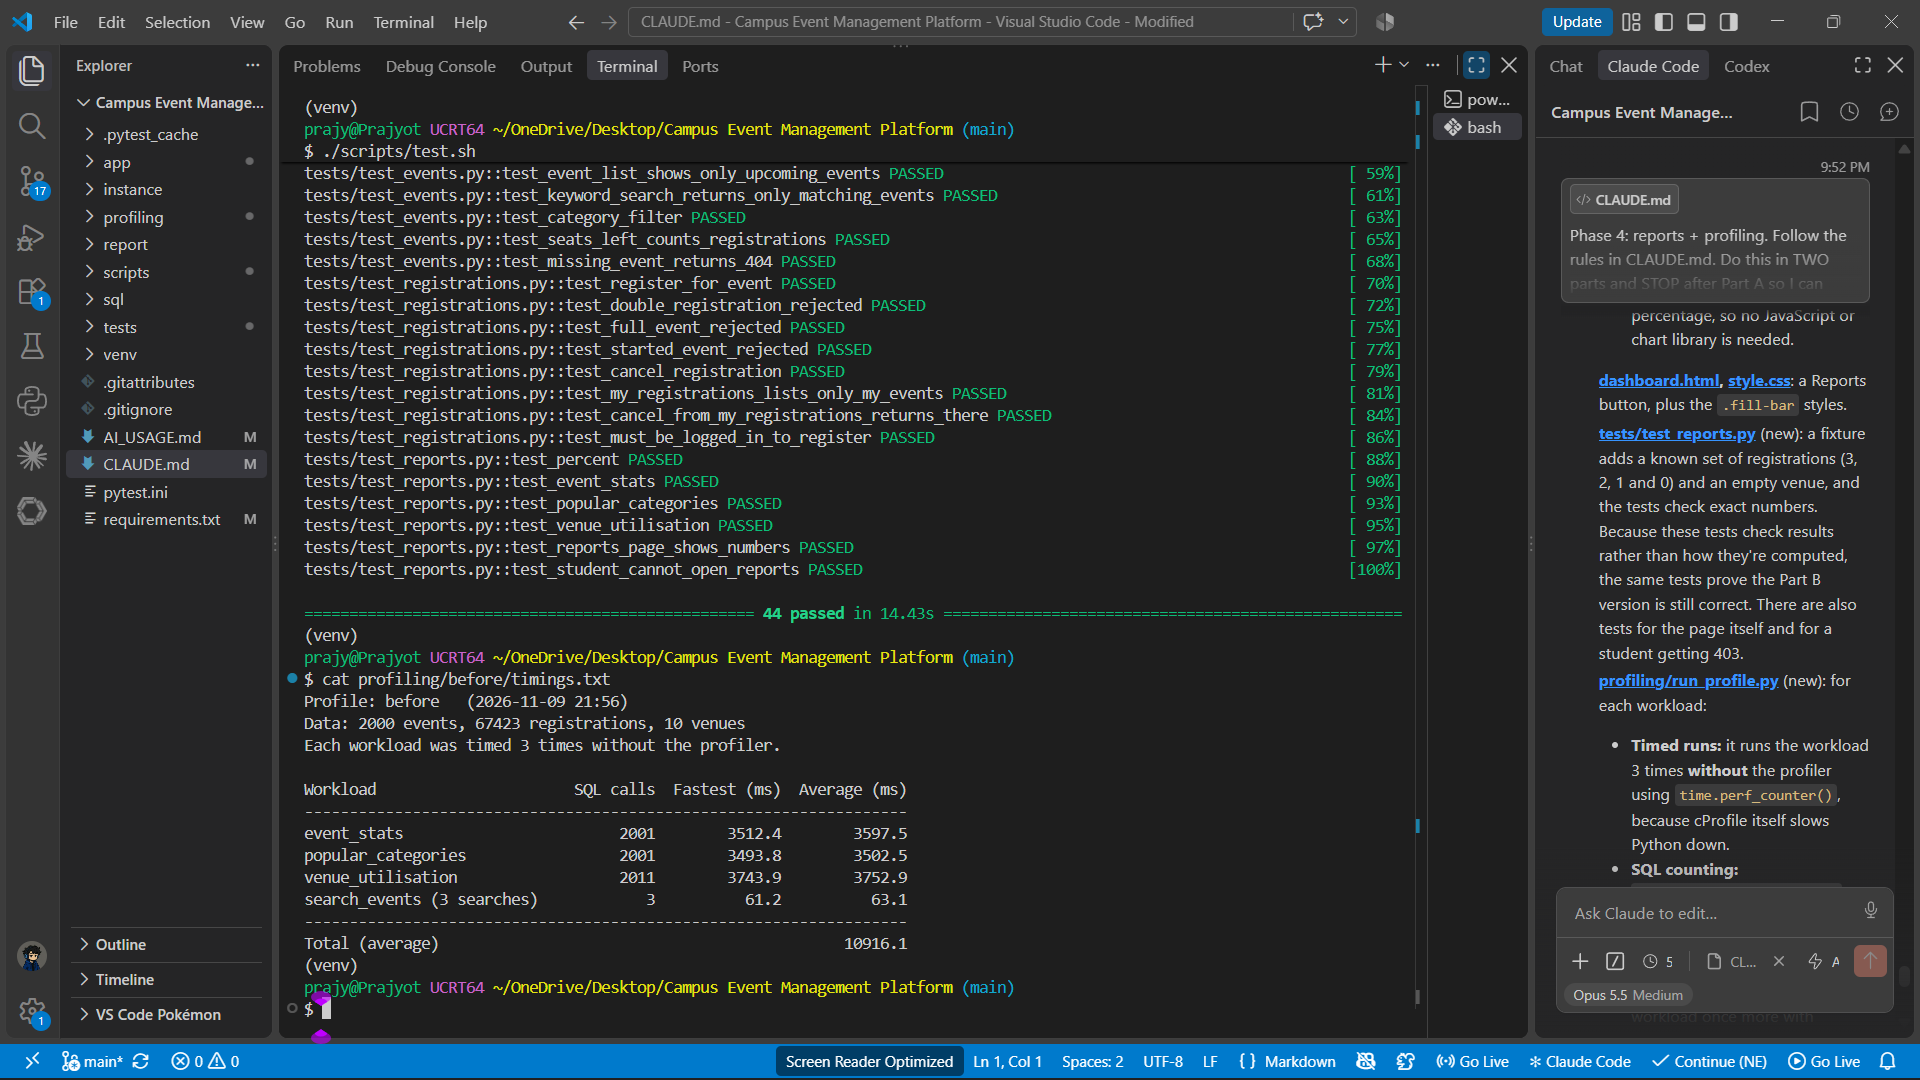
\includegraphics[width=0.9\linewidth]{figures/reports_page.png}
\caption{Running \texttt{./scripts/test.sh} in Git Bash (taken during the profiling phase, when
there were 44 tests), followed by the baseline \texttt{timings.txt}.}
\end{figure}

% =====================================================================
\section{Profiling and optimisation}
\label{sec:profiling}

\subsection{Method}

The reports page was first written the naive way on purpose, and then measured.
\code{scripts/profile.sh} builds a separate database (\code{profiling/profile.db}, selected
with the \code{CAMPUS_DB} environment variable so the demo data is never touched) and seeds it with
\textbf{2000 events, 67{,}423 registrations, 10 venues and 100 students} using fixed random seeds,
so every run uses the same data. \code{profiling/run_profile.py} then, for each workload:

\begin{enumerate}[itemsep=2pt]
  \item runs it three times \emph{without} the profiler and records the wall-clock time with
        \code{time.perf_counter()} (cProfile itself slows Python down);
  \item counts the SQL statements one run sends, using \code{sqlite3}'s
        \code{set_trace_callback};
  \item runs it once more under \code{cProfile} and saves \code{profile.prof} plus a
        \code{pstats} summary sorted by cumulative time.
\end{enumerate}

The workloads are the three report functions and three typical event searches.
\code{profiling/explain.py} also records \code{EXPLAIN QUERY PLAN} for the important queries.

\subsection{The bottleneck: the N+1 query problem}

The naive report code fetched all events and then ran one \code{COUNT} query per event:

\begin{lstlisting}[language=Python, caption={Naive version (first commit of app/reports.py).}]
def count_registrations(event_id):
    """How many students registered for one event. ONE SQL query per call."""
    return get_db().execute(
        "SELECT COUNT(*) FROM registrations WHERE event_id = ?", (event_id,)
    ).fetchone()[0]

def event_stats():
    events = get_db().execute("SELECT id, title, ... FROM events").fetchall()
    for event in events:
        registered = count_registrations(event["id"])   # N+1: one query per event
        ...
\end{lstlisting}

The top of the \code{cProfile} output made the problem obvious:

\begin{verbatim}
         86185 function calls in 10.646 seconds
   ncalls  tottime  percall  cumtime  percall filename:lineno(function)
     6000    0.020    0.000   10.540    0.002 reports.py:21(count_registrations)
     6016   10.479    0.002   10.479    0.002 {method 'execute' of 'sqlite3.Connection'}
        1    0.010    0.010    3.574    3.574 reports.py:28(event_stats)
        1    0.005    0.005    3.511    3.511 reports.py:75(venue_utilisation)
        1    0.008    0.008    3.496    3.496 reports.py:56(popular_categories)
        3    0.000    0.000    0.063    0.021 events.py:52(search_events)
\end{verbatim}

\code{count_registrations} was called 6000 times (2000 per report) and accounts for 10.54 of the
10.65 seconds, which is 99\%. Almost all of that is \emph{tottime} inside SQLite's \code{execute},
not in our Python code. The problem was not slow Python. It was \textbf{too many queries, each doing
too much work}. \code{EXPLAIN QUERY PLAN} showed why each query was slow:

\begin{verbatim}
SCAN registrations USING COVERING INDEX sqlite_autoindex_registrations_1
\end{verbatim}

The only index on \code{registrations} came from \code{UNIQUE(user_id, event_id)}. It starts
with \code{user_id}, so it cannot help \code{WHERE event_id = ?}, and SQLite read all 67{,}423
entries for every single count: roughly $2000 \times 67{,}423 \approx 135$ million entries per report.

\begin{figure}[H]
\centering
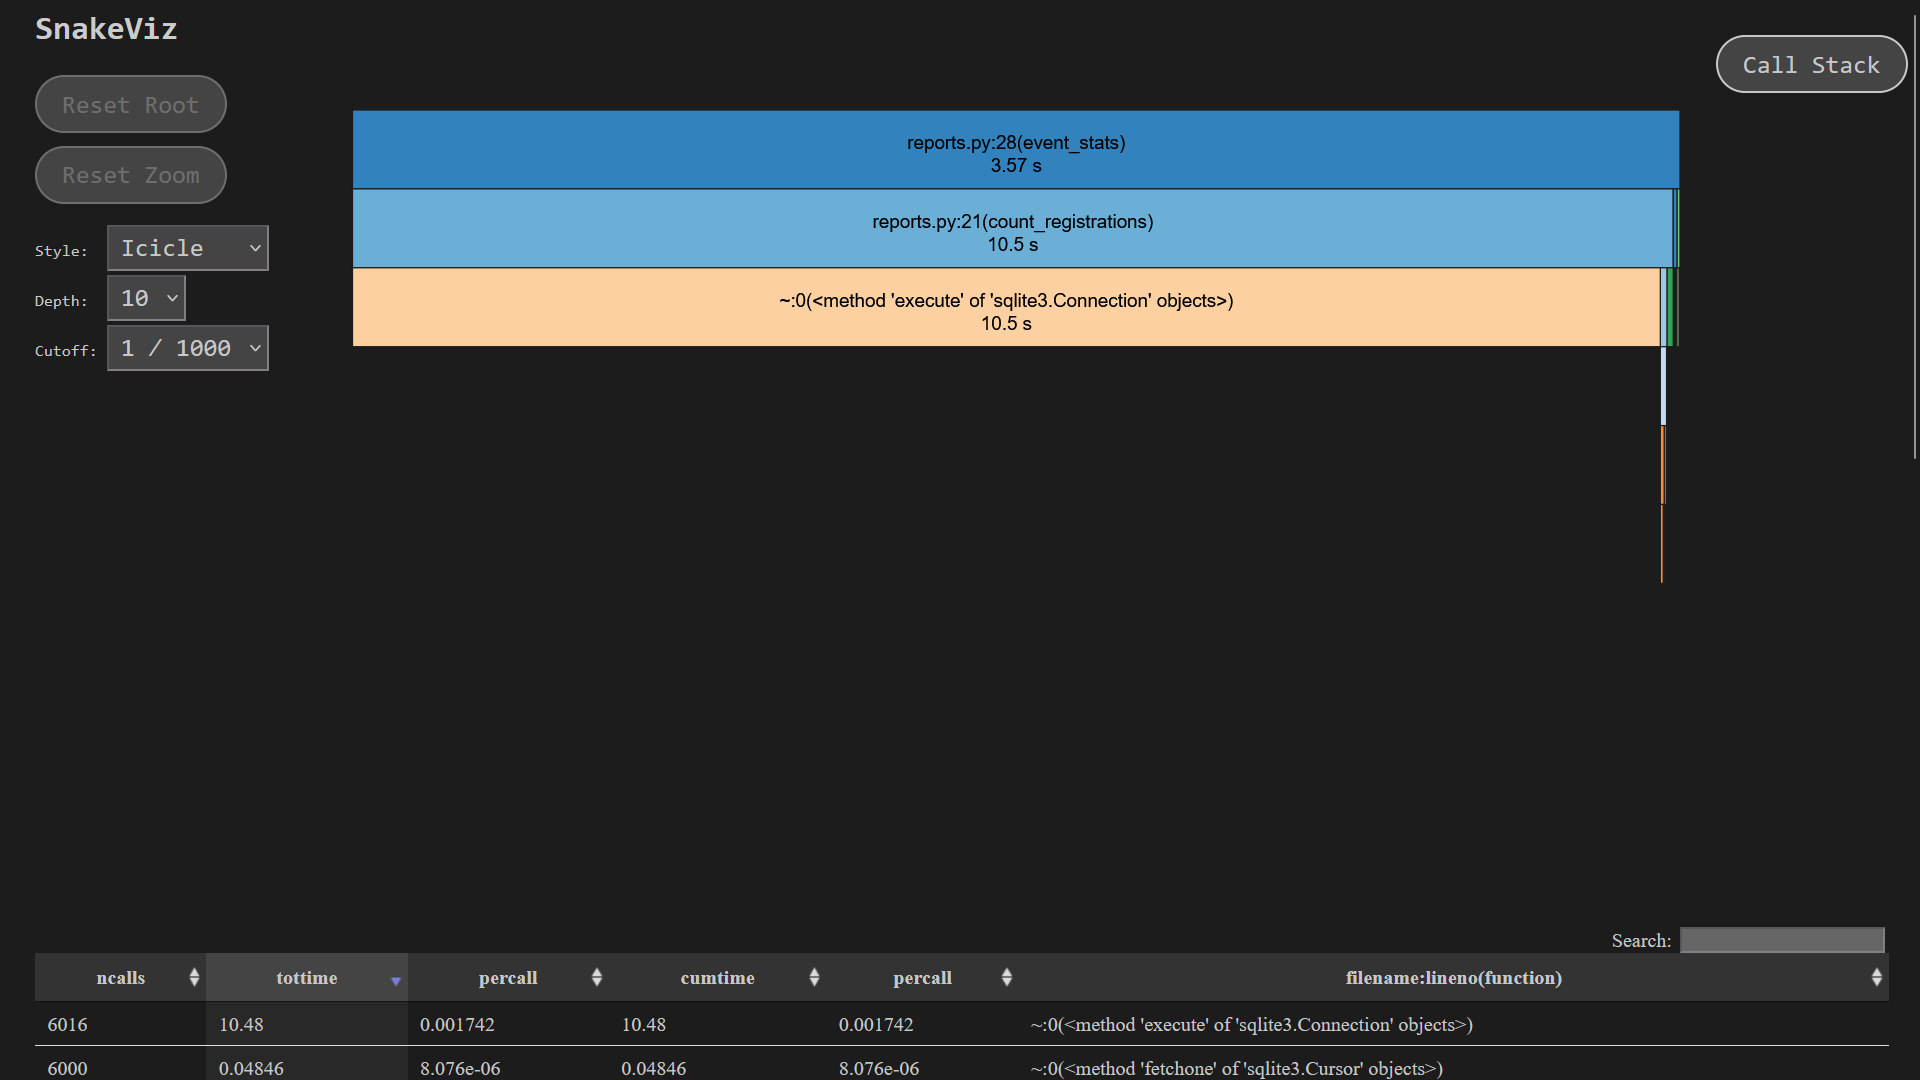
\includegraphics[width=0.9\linewidth]{figures/before_snakeviz.png}
\caption{SnakeViz icicle chart of the \emph{before} profile: \texttt{event\_stats} (3.57\,s) is
almost entirely \texttt{count\_registrations} $\rightarrow$ \texttt{sqlite3 execute} (10.5\,s in total).}
\end{figure}

\begin{figure}[H]
\centering
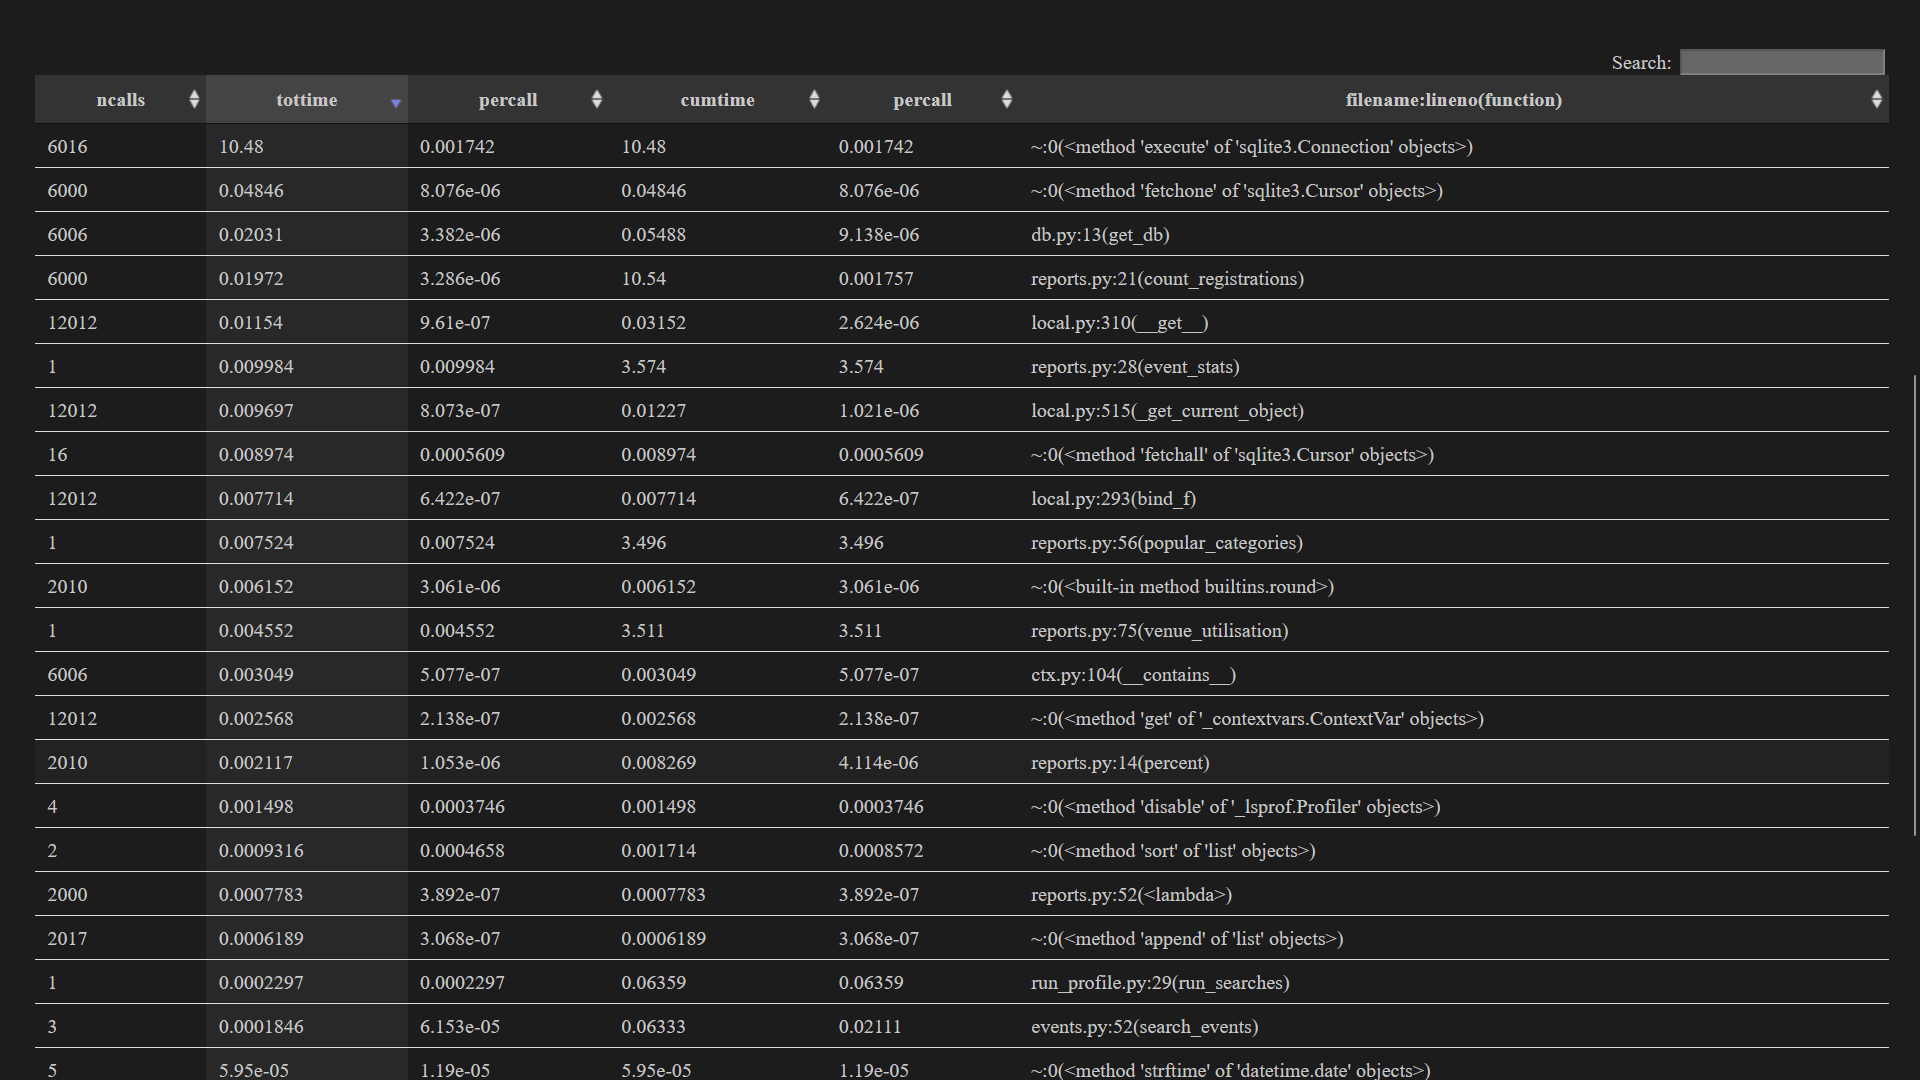
\includegraphics[width=0.9\linewidth]{figures/snakeviz.png}
\caption{SnakeViz table of the \emph{before} profile, sorted by own time: 6016 calls to
\texttt{execute} take 10.48\,s.}
\end{figure}

\subsection{The fixes}

\paragraph{1. One query per report.} Each report became a single query using \code{LEFT JOIN}
and \code{GROUP BY}, so the database counts everything in one pass. \code{LEFT JOIN} keeps events
with no registrations (their count is 0). For the categories report, \code{COUNT(DISTINCT e.id)}
is needed because the join repeats each event once per registration. For venue utilisation, an inner
query first counts registrations per event; otherwise \code{SUM(capacity)} would be multiplied by
the number of registrations. Percentages are still rounded in Python by the same \code{percent()}
function, because Python and SQLite round halves differently.

\begin{lstlisting}[language=SQL, caption={Optimised event\_stats query (app/reports.py).}]
SELECT e.id, e.title, e.category, e.start_time, e.capacity,
       COUNT(r.id) AS registered
FROM events e
LEFT JOIN registrations r ON r.event_id = e.id
GROUP BY e.id
ORDER BY registered DESC, e.start_time, e.id
\end{lstlisting}

\paragraph{2. Indexes.} \code{sql/indexes.sql} adds three indexes, applied by \code{setup.sh}
and \code{profile.sh}:

\begin{lstlisting}[language=SQL, caption={sql/indexes.sql (comments shortened).}]
-- counting / joining registrations per event
CREATE INDEX IF NOT EXISTS idx_registrations_event ON registrations (event_id);
-- venue filter on the search page and the clash check
CREATE INDEX IF NOT EXISTS idx_events_venue_start ON events (venue_id, start_time);
-- category dropdown on the search page
CREATE INDEX IF NOT EXISTS idx_events_category    ON events (category);
\end{lstlisting}

An index on \code{registrations(user_id)} was considered and \emph{not} added: the
\code{UNIQUE(user_id, event_id)} constraint already gives SQLite an index whose leftmost column
is \code{user_id}, and the query plan for \code{WHERE user_id = ? AND event_id = ?} already uses it.
A second index would only slow down writes.

\subsection{Results}

\begin{table}[H]
\centering
\small
\begin{tabular}{@{}l r r r r r r@{}}
\toprule
& \multicolumn{2}{c}{\textbf{SQL calls}} & \multicolumn{3}{c}{\textbf{Average time (ms)}} & \\
\cmidrule(lr){2-3}\cmidrule(lr){4-6}
\textbf{Workload} & \textbf{before} & \textbf{after} & \textbf{before} & \textbf{rewrite only} & \textbf{after} & \textbf{Speed-up} \\
\midrule
\code{event_stats}        & 2001 & 1 & 3597.5 & 22.9 & 9.1  & $\approx 395\times$ \\
\code{popular_categories} & 2001 & 1 & 3502.5 & 36.0 & 6.5  & $\approx 539\times$ \\
\code{venue_utilisation}  & 2011 & 1 & 3752.9 & 19.8 & 6.0  & $\approx 625\times$ \\
\code{search_events} (3 searches) & 3 & 3 & 63.1 & 66.0 & 10.9 & $\approx 5.8\times$ \\
\midrule
\textbf{Total} & \textbf{6016} & \textbf{6} & \textbf{10916.1} & \textbf{144.7} & \textbf{32.6} & $\mathbf{\approx 335\times}$ \\
\bottomrule
\end{tabular}
\caption{Before and after, 2000 events and 67{,}423 registrations. \emph{Rewrite only} = new
queries without indexes (\texttt{APPLY\_INDEXES=0 ./scripts/profile.sh rewrite\_only}).}
\label{tab:results}
\end{table}

\begin{figure}[H]
\centering
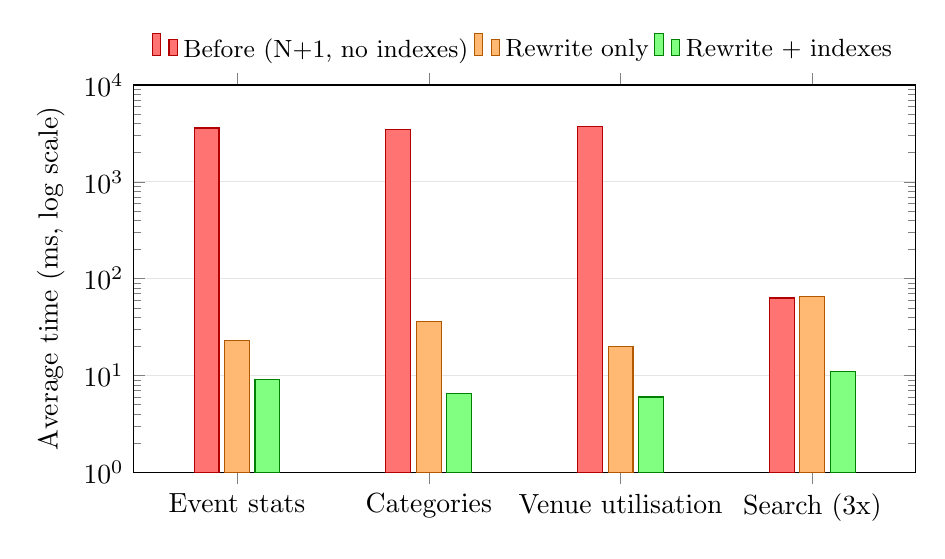
\begin{tikzpicture}
\begin{axis}[
    ybar, ymode=log, log origin=infty,
    width=0.95\linewidth, height=6.5cm,
    bar width=9pt,
    ymin=1, ymax=10000,
    ylabel={Average time (ms, log scale)},
    xtick={1,2,3,4},
    xticklabels={Event stats, Categories, Venue utilisation, Search (3x)},
    enlarge x limits=0.18,
    ymajorgrids, grid style={black!10},
    legend style={at={(0.5,1.03)}, anchor=south, legend columns=3, draw=none, font=\small},
  ]
  \addplot[fill=red!55, draw=red!70!black]     coordinates {(1,3597.5) (2,3502.5) (3,3752.9) (4,63.1)};
  \addplot[fill=orange!55, draw=orange!70!black] coordinates {(1,22.9) (2,36.0) (3,19.8) (4,66.0)};
  \addplot[fill=green!50, draw=green!50!black] coordinates {(1,9.1) (2,6.5) (3,6.0) (4,10.9)};
  \legend{{Before (N+1, no indexes)}, {Rewrite only}, {Rewrite + indexes}}
\end{axis}
\end{tikzpicture}
\caption{Average time per workload. Note the logarithmic scale: each grid line is 10$\times$.}
\end{figure}

After the changes, \code{execute} is called 6 times and takes 0.026\,s in total (it was 6016 calls
and 10.48\,s), and the profiled run makes 6{,}139 function calls instead of 86{,}185. An extra
measurement of the \emph{old} N+1 loop on the \emph{indexed} database took about 115\,ms. So the
indexes alone give about $31\times$, the rewrite alone about $157\times$, and both together about
$395\times$ for \code{event_stats}. Each fix helps, and they work better together.

\begin{figure}[H]
\centering
\screenshot{figures/after_snakeviz.png}{0.9\linewidth}{snakeviz profiling/after/profile.prof, icicle view}
\caption{SnakeViz view of the \emph{after} profile.}
\end{figure}

\subsection{Query plans}

\code{EXPLAIN QUERY PLAN} shows how SQLite runs a query. \code{SCAN} means reading every row;
\code{SEARCH ... USING INDEX} means jumping straight to the matching rows; \code{AUTOMATIC ...
INDEX} means SQLite had to build a temporary index for this one query and throw it away afterwards,
which is a sign that a permanent index is missing.

\paragraph{Event search, no filters} (the main events page):
\begin{verbatim}
BEFORE                                     AFTER
SCAN e                                     SCAN e
SEARCH v USING INTEGER PRIMARY KEY         SEARCH v USING INTEGER PRIMARY KEY
BLOOM FILTER ON r (event_id=?)
SEARCH r USING AUTOMATIC COVERING INDEX    SEARCH r USING COVERING INDEX
         (event_id=?) LEFT-JOIN                     idx_registrations_event
                                                    (event_id=?) LEFT-JOIN
USE TEMP B-TREE FOR ORDER BY               USE TEMP B-TREE FOR ORDER BY
\end{verbatim}
Before, SQLite built a temporary index over all 67{,}000 registrations \emph{on every search}.
After, it uses the permanent index, which explains 63\,ms $\rightarrow$ 11\,ms.

\paragraph{Other queries:}
\begin{verbatim}
Per-event COUNT (naive report, run ~2000 times):
  before: SCAN registrations USING COVERING INDEX sqlite_autoindex_registrations_1
  after:  SEARCH registrations USING COVERING INDEX idx_registrations_event (event_id=?)
Search with category + date range:
  before: SCAN e
  after:  SEARCH e USING INDEX idx_events_category (category=?)
Search with venue filter:
  before: SCAN e
  after:  SEARCH e USING INDEX idx_events_venue_start (venue_id=? AND start_time>?)
Venue clash check:
  before: SCAN events
  after:  SEARCH events USING INDEX idx_events_venue_start (venue_id=? AND start_time<?)
\end{verbatim}

\subsection{Why it got faster, and what did not change}

\begin{enumerate}[itemsep=2pt]
  \item \textbf{Fewer round trips.} Every \code{execute()} has a fixed cost (Python to SQLite,
        preparing the statement, building result objects). 6016 calls became 6.
  \item \textbf{Less data read per query.} An index is a sorted copy of a column with pointers
        back to the rows, like the index of a book. With it, SQLite finds one event's
        registrations in $O(\log n)$ steps instead of reading all $n$ rows.
  \item \textbf{No throw-away work.} The temporary \code{AUTOMATIC} indexes are no longer
        rebuilt for each query.
  \item \textbf{Covering index.} \code{idx_registrations_event} contains everything a count
        needs, so SQLite never reads the registrations table itself.
\end{enumerate}

Some things did not change. A keyword search still scans all events, because
\texttt{LIKE '\%workshop\%'} starts with a wildcard and an ordinary index cannot help (like looking up
every word that \emph{contains} ``shop'' in a dictionary); SQLite's full-text search (FTS5) would be
needed. Indexes are not free either: every \code{INSERT} or \code{DELETE} must also update them
and the database file grows a little. Because this app reads far more often than it writes, the
trade-off is worth it.

% =====================================================================
\section{Git workflow}

The project was developed in phases, with all commits made by the author on the \code{main}
branch. Each commit is small, does one thing, and leaves the project in a working state where the
tests pass. Commit messages follow the Conventional Commits style:

\begin{table}[H]
\centering
\small
\begin{tabular}{@{}l l r@{}}
\toprule
\textbf{Prefix} & \textbf{Meaning} & \textbf{Commits} \\
\midrule
\code{feat:}  & a new feature                        & 10 \\
\code{test:}  & adding or changing tests             & 3 \\
\code{perf:}  & a performance improvement            & 2 \\
\code{chore:} & setup, tooling, scripts              & 3 \\
\code{docs:}  & documentation, notes and results     & 5 \\
\midrule
\textbf{Total} (before this documentation phase) & & \textbf{23} \\
\bottomrule
\end{tabular}
\caption{Commit types.}
\end{table}

\begin{table}[H]
\centering
\small
\begin{tabularx}{\linewidth}{@{}l r X@{}}
\toprule
\textbf{Phase} & \textbf{Commits} & \textbf{Example commit messages} \\
\midrule
1. Skeleton           & 5 & \code{chore: set up project structure and dependencies}; \code{feat: add SQLite schema for users, venues, events, registrations} \\
2. Auth and browsing  & 6 & \code{feat: add student registration, login and logout with Flask-Login}; \code{test: add pytest fixtures and auth/event tests} \\
3. Registrations and admin & 5 & \code{feat: let students register for and cancel events}; \code{feat: add admin CRUD for venues and events with clash check and CSV export} \\
4a. Naive reports + baseline & 3 & \code{feat: add admin reports page (naive N+1 version) with tests}; \code{docs: record baseline profile of naive reports} \\
4b. Optimisation      & 4 & \code{perf: replace N+1 report loops with JOIN + GROUP BY queries}; \code{perf: add database indexes and apply them in setup and profiling} \\
\bottomrule
\end{tabularx}
\caption{History summary (\texttt{git log --oneline}).}
\end{table}

Two habits made the history useful. First, the naive reports and their baseline measurements were
committed \emph{before} the optimisation, so the history itself proves what was measured and when.
Second, \code{.gitignore} keeps build and environment files (the virtual environment, \code{*.db},
\code{__pycache__}, LaTeX build files) out of the repository, and \code{.gitattributes} forces
\code{.sh} files to use Unix line endings, so a Windows checkout cannot break the Bash scripts with
\verb|$'\r': command not found|.

% =====================================================================
\section{AI usage declaration}
\label{sec:ai}

I used Claude, an AI assistant made by Anthropic (through the Claude Code extension in VS Code),
during this project.

\paragraph{What it was used for.} Drafting much of the application code, Bash scripts, tests and
documentation from my specifications (the features, the database schema, raw SQL without an ORM,
and a naive first version of the reports to be profiled and then optimised); explaining concepts and
code, such as Flask Blueprints, cProfile output, query plans and indexes; and helping diagnose
problems and suggest improvements, including the Windows \code{flask.exe} launcher issue, the Jinja
comment bug and the redundant \code{registrations(user_id)} index.

\paragraph{What I did.} I defined the requirements and the order of work. I ran every script and the
full test suite myself in Git Bash on Windows and tested the features in the browser. I reviewed all
of the code and every suggestion before accepting it, including the decision to leave out the
redundant index. I ran the profiling, took the screenshots and made every git commit myself.
A phase-by-phase log is in \code{AI_USAGE.md} in the repository.

\paragraph{In my own words.}
\todo{Write 3--5 sentences yourself: what you learned, what you checked or changed by hand, and
anything you did differently from the suggestions. Keep it consistent with AI\_USAGE.md.}

% =====================================================================
\section{Challenges}

\paragraph{Windows: \texttt{flask.exe} ``Permission denied''.} The first run of \code{setup.sh}
failed when Git Bash tried to start the \code{flask.exe} launcher inside the virtual environment.
Running Flask as a module, \code{python -m flask --app app ...}, avoids the launcher entirely and works
the same on every operating system, so every script uses it. A related trap was that \code{python3}
on Windows can be a Microsoft Store shortcut that exists but does not work, which is why
\code{find_python} runs \code{--version} instead of only checking that the command exists.

\paragraph{Jinja parses tags inside HTML comments.} The base template contained the HTML comment
\verb|<!-- Each page can set its own title with {% block title %} -->|. The browser would ignore
it, but Jinja processes the template first, saw a real \verb|{% block %}| tag and failed with
``Unexpected end of template''. The fix is to use Jinja's own comment syntax, \verb|{# ... #}|,
for comments that mention template tags.

\paragraph{Which indexes to add.} The plan listed an index on \code{registrations(user_id)}.
Checking the query plans showed that the \code{UNIQUE(user_id, event_id)} constraint already
creates an index starting with \code{user_id}, which the ``is this student registered?'' query
already uses. Adding another would cost disk space and slow down every registration while making
no query faster, so it was left out and the reason documented in \code{sql/indexes.sql}.

\paragraph{The last-seat race condition.} Registration checks the seats left and then inserts in
two separate statements. If two students click \emph{Register} for the last seat at almost the same
moment, both checks could see one seat left before either insert happens, and the event would be
over-booked by one. At demo scale this is practically impossible, but the proper fix is to make the
check and the insert one atomic step: for example, a single
\code{INSERT ... SELECT ... WHERE (SELECT COUNT(*) ...) < capacity} and checking whether a row
was inserted, or wrapping both in a \code{BEGIN IMMEDIATE} transaction.

\paragraph{A failing test that was the test's fault.} The first version of the clash-check test
used a time window starting in the year 2000 and expected no clash. It failed, because that window
really did overlap a past event at the same venue in the sample data. The application was right and
the test was wrong; the test now uses a one-hour window just before the event.

% =====================================================================
\section{Conclusion and future work}

The Campus Event Management Platform meets its objectives. Students can find and register for
events, admins can manage events and venues without double-booking a room, and reports show how
events and venues are used. The project combines HTML/CSS, Python, SQL, Git, Bash and LaTeX; it is
covered by 45 automated tests; and profiling found a real bottleneck, the N+1 query problem made
worse by a missing index, whose fix made the reports about 335 times faster without changing a
single reported number.

The main lesson was to \emph{measure before optimising}: the profiler showed that the cost was in
the number and kind of SQL queries, not in Python, and \code{EXPLAIN QUERY PLAN} showed exactly
which index was missing.

\paragraph{Future work.}
\begin{itemize}[itemsep=2pt]
  \item Make registration atomic to remove the last-seat race condition.
  \item CSRF tokens on forms (for example with Flask-WTF) in addition to \code{SameSite} cookies.
  \item Full-text search (SQLite FTS5) so keyword search can use an index.
  \item Pagination for the event list and reports, email confirmations and reminders, and a
        waiting list when an event is full.
  \item Deployment with a production WSGI server and a real secret key.
\end{itemize}

% =====================================================================
\begin{thebibliography}{99}
\bibitem{flask} Pallets Projects. \emph{Flask documentation}. \url{https://flask.palletsprojects.com/}
\bibitem{flasklogin} \emph{Flask-Login documentation}. \url{https://flask-login.readthedocs.io/}
\bibitem{werkzeug} Pallets Projects. \emph{Werkzeug: security helpers}. \url{https://werkzeug.palletsprojects.com/}
\bibitem{sqlite-planner} SQLite. \emph{The SQLite query optimizer overview} and \emph{EXPLAIN QUERY PLAN}. \url{https://www.sqlite.org/optoverview.html}, \url{https://www.sqlite.org/eqp.html}
\bibitem{sqlite-index} SQLite. \emph{CREATE INDEX} and \emph{automatic indexes}. \url{https://www.sqlite.org/lang_createindex.html}
\bibitem{pysqlite} Python Software Foundation. \emph{sqlite3: DB-API 2.0 interface for SQLite databases}. \url{https://docs.python.org/3/library/sqlite3.html}
\bibitem{cprofile} Python Software Foundation. \emph{The Python profilers (cProfile, pstats)}. \url{https://docs.python.org/3/library/profile.html}
\bibitem{snakeviz} \emph{SnakeViz}. \url{https://jiffyclub.github.io/snakeviz/}
\bibitem{pytest} \emph{pytest documentation}. \url{https://docs.pytest.org/}
\bibitem{faker} \emph{Faker documentation}. \url{https://faker.readthedocs.io/}
\bibitem{progit} S. Chacon and B. Straub. \emph{Pro Git}, 2nd ed., Apress. \url{https://git-scm.com/book}
\bibitem{cc} \emph{Conventional Commits 1.0.0}. \url{https://www.conventionalcommits.org/}
\bibitem{bash} GNU. \emph{Bash Reference Manual}. \url{https://www.gnu.org/software/bash/manual/}
\bibitem{tikz} T. Tantau. \emph{The TikZ and PGF Packages: Manual}. \url{https://ctan.org/pkg/pgf}
\end{thebibliography}

\end{document}
